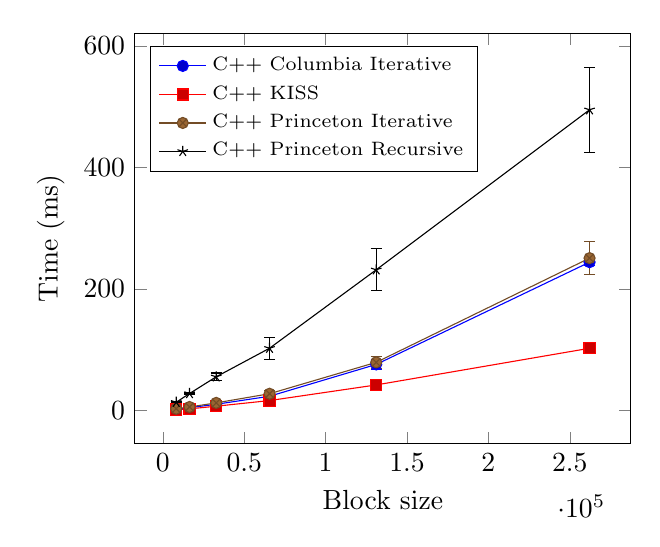
\begin{tikzpicture}
\begin{axis}[xlabel={Block size},ylabel={Time (ms)},width=0.65\linewidth,legend pos=north west,scaled y ticks = false,legend cell align=left,legend style={font=\scriptsize}]
\addplot+[error bars/.cd, y dir=both,y explicit] coordinates {
(8192, 1.9326) +- (0.2654, 0.2654)
(16384, 4.2789) +- (0.6399, 0.6399)
(32768, 9.9388) +- (1.6341, 1.6341)
(65536, 23.1031) +- (3.9019, 3.9019)
(131072, 75.4942) +- (8.3819, 8.3819)
(262144, 243.8496) +- (5.1390, 5.1390)
};
\addplot+[error bars/.cd, y dir=both,y explicit] coordinates {
(8192, 1.2470) +- (0.2301, 0.2301)
(16384, 2.3713) +- (0.4915, 0.4915)
(32768, 6.7420) +- (1.2931, 1.2931)
(65536, 16.0281) +- (1.8073, 1.8073)
(131072, 41.7620) +- (3.0449, 3.0449)
(262144, 102.1196) +- (5.5195, 5.5195)
};
\addplot+[error bars/.cd, y dir=both,y explicit] coordinates {
(8192, 2.5845) +- (0.2085, 0.2085)
(16384, 5.4518) +- (0.5858, 0.5858)
(32768, 12.2266) +- (2.4651, 2.4651)
(65536, 27.2805) +- (4.8616, 4.8616)
(131072, 78.9501) +- (9.8472, 9.8472)
(262144, 250.4870) +- (26.9237, 26.9237)
};
\addplot+[error bars/.cd, y dir=both,y explicit] coordinates {
(8192, 13.2345) +- (0.7311, 0.7311)
(16384, 27.6080) +- (0.9098, 0.9098)
(32768, 55.1227) +- (6.2636, 6.2636)
(65536, 102.1585) +- (17.9911, 17.9911)
(131072, 231.2663) +- (34.3656, 34.3656)
(262144, 494.7038) +- (69.7402, 69.7402)
};
\legend{C++ Columbia Iterative , C++ KISS , C++ Princeton Iterative , C++ Princeton Recursive}
\end{axis}
\end{tikzpicture}
